\documentclass[11pt]{article}

\usepackage[margin=1in]{geometry}
\usepackage{amsmath,amssymb}
\usepackage{graphicx}
\usepackage{booktabs}
\usepackage{array}
\usepackage[numbers,sort&compress]{natbib}
\usepackage{hyperref}
\usepackage{caption}
\usepackage{subcaption}
\usepackage{placeins}

\emergencystretch=2em

\title{\textbf{QALBench: A Tiered Audit Benchmark and Reference Implementation for Quantum Artificial-Life Claims}\\
\large Population Lineages, Classical Controls, and Quantum-Resource Ablations}
\author{Gabriel Kahen\thanks{Corresponding author: \href{mailto:gabekahen@gmail.com}{gabekahen@gmail.com}.}\\Independent Researcher\\United States}
\date{May 2026}

\newcommand{\ket}[1]{\left|#1\right\rangle}
\newcommand{\bra}[1]{\left\langle#1\right|}
\newcommand{\Tr}{\operatorname{Tr}}
\newcommand{\sx}{\sigma_x}
\newcommand{\sy}{\sigma_y}
\newcommand{\sz}{\sigma_z}
\newcommand{\MI}{I}
\newcolumntype{P}[1]{>{\raggedright\arraybackslash}p{#1}}

\begin{document}
\maketitle

\begin{abstract}
Quantum artificial-life (QAL) papers often combine artificial-life labels, such as inheritance, mutation, interaction, turnover, and selection, with quantum-resource labels, such as coherence, entanglement, Bell nonlocality, and channel resources. These labels require different records and different controls. This paper introduces QALBench as a tiered audit benchmark with a reference implementation, not as a leaderboard or a detector of new QAL phenomena. The protocol separates artificial-life adequacy, quantum-resource evidence, and computational nonclassicality.

The benchmark defines a task ladder that ranges from basis-inheritance and mutation-channel checks through resource diagnostics, population lineage audits, resource-coupled outcome controls, finite-shot certification workflows, and computational-nonclassicality submissions. The suite implementation defines auditable task families across T1--T6, while the checked-in numerical reference experiments remain conservative T1--T4 demonstrations. A cloned-observable resource kernel compares an exact two-qubit density-matrix simulation, a stepwise dephased simulation, and a matched classical Markov chain. For this implemented event family and measurement basis, computational-basis inheritance probabilities are fixed by a diagonal transition map, while off-diagonal coherence, negativity, concurrence, and the Horodecki value for possible CHSH violation identify state resources removed by the dephased and Markov controls. A population module adds lineage-audited records for identities, parent--offspring events, inherited continuous genotype parameters, expressed computational-basis phenotypes, births, deaths, mutations, interaction exposure, imposed selection rules, no-inheritance controls, and shuffled-lineage diagnostics.

The population experiments are reporting and control checks, not a new quantum artificial-life phenomenon. Under matched seeds, basis-selection demographic, phenotype, and lineage summaries are identical for the quantum, dephased, and classical controls, excluding resource diagnostics. A software positive-control assay intentionally inserts a stored negativity-derived birth-event score into the reproduction rule and shows how such synthetic scalar feedback is removed by dephasing or Markov controls. A no-inheritance resource control remains resource-positive but transmission-negative, showing that resource-coupled reproduction is not the same as inherited resource-mediated artificial life. QALBench supplies hardware-ready finite-shot and simulator-challenge verification workflows, but its included reference packages do not claim quantum advantage, loophole-free hardware certification, open-ended evolution, or persistent population-level entanglement.
\end{abstract}

\section{Introduction}

Artificial life studies synthetic systems that reproduce, vary, interact, adapt, and sometimes sustain open-ended novelty \citep{vonneumann1966self,bedau2003artificial,ray1992tierra,ofria2004avida,lenski2003evolutionary,bullock2006exploring,banzhaf2016defining,packard2019overview,dolson2019modes}. Quantum information studies resources that cannot be reduced to a classical probability distribution over mutually compatible properties \citep{wootters1982single,barnum1996noncommuting,bell1964einstein,clauser1969proposed,chitambar2019quantum}. A quantum artificial-life experiment can therefore succeed in several distinct ways. It can implement life-like dynamics on quantum hardware. It can preserve and certify a quantum resource during those dynamics. Or, more strongly, it can define a scalable task whose output resists known efficient classical simulations.

Those are different claims. A population model with excellent inheritance, mutation, selection, and turnover can still be classical. A two-qubit Bell pair can be strongly quantum while doing no artificial life. A small entangled circuit can also remain efficiently classically simulable. The problem for QAL reporting is not that any one label is illegitimate. The problem is that the labels are often reported with the wrong controls.

The Alvarez-Rodriguez--Sanz--Lamata--Solano program makes the issue concrete. The 2014 biomimetic-cloning protocol copies a selected observable without cloning an arbitrary unknown state \citep{alvarez2014biomimetic}. The 2016 QAL model represents each individual with genotype and phenotype qubits and adds self-replication, mutation, interaction, and Lindblad aging/death \citep{alvarez2016artificial,lindblad1976generators}. The 2018 IBM implementation reports small QAL subprotocols on superconducting hardware and explicitly distinguishes computational-basis inheritance from cross-generational quantum correlations \citep{alvarez2018ibm}. Later theoretical work explores thermodynamic self-replication mechanisms in light--matter systems \citep{valente2021self,lamata2020perspective}. Adjacent quantum cellular-automaton and quantum Game-of-Life work studies quantum many-body or circuit analogues of cellular rules rather than lineage-audited QAL claims \citep{bleh2012quantum,ney2022entanglement,escanez2026qgol}. These papers are valuable, but they also show why a benchmark must ask claim-specific questions: what was inherited, what varied, what turned over, what was selected, what was measured in noncommuting settings, and what classical control failed?

QALBench is designed around that separation. It contains a tiered task suite, a reporting schema, two implemented numerical reference modules, and reusable submission, verification, and scoring workflows. The tiers make partial results reportable without implying stronger claims: a study can pass a basis-inheritance task without passing a resource-dependence task, or pass a resource-diagnostic task without earning a population-level artificial-life claim. The first numerical module is the cloned-observable resource kernel: it tests when basis-probability inheritance data are reproduced by dephased and Markov controls and where noncommuting quantum diagnostics remain. The second numerical module is a population audit module: it computes individual, parent--child, inherited genotype-parameter, expressed-phenotype, birth, death, mutation, interaction-exposure, selection-rule, and resource-ablation records, then reports summary and time-series artifacts. The suite layer extends these examples with finite-shot certificate validators, simulator-baseline manifests, and independent axis scoring. The reference implementation is intentionally conservative. It does not equate artificial-life adequacy with quantum resources, and it does not equate quantum resources with computational advantage.

\subsection{Related Work and Gap}

QALBench draws from four literatures whose standards are often mixed together in QAL discussions. First, artificial-life systems such as self-reproducing automata, Tierra, Avida, and digital-evolution models establish that inheritance, mutation, turnover, selection, diversity, and open-endedness are population claims requiring explicit records, not labels inferred from the presence of update rules \citep{vonneumann1966self,ray1992tierra,ofria2004avida,lenski2003evolutionary,bedau2003artificial,bullock2006exploring,banzhaf2016defining,packard2019overview,dolson2019modes}. Second, the QAL and quantum-biomimetics literature provides cloned-observable inheritance, genotype--phenotype circuits, quantum-correlation diagnostics, hardware demonstrations, and thermodynamic replication mechanisms \citep{alvarez2014biomimetic,alvarez2016artificial,alvarez2018ibm,lamata2020perspective,valente2021self}. Third, quantum cellular-automaton and quantum Game-of-Life studies explore many-body or grid-rule analogues that are adjacent to, but not identical with, lineage-audited artificial-life claims \citep{bleh2012quantum,ney2022entanglement,escanez2026qgol}. Fourth, quantum-information, coherence-resource, certification, and quantum-benchmarking work supplies the resource diagnostics, Bell-test assumptions, tomography cautions, and classical-simulation baselines needed before resource or computational-nonclassicality language is justified \citep{bell1964einstein,clauser1969proposed,baumgratz2014coherence,horodecki1995violating,guhne2009entanglement,brunner2014bell,li2020qasmbench,tomesh2022supermarq,gottesman1998heisenberg,aaronson2004improved,vidal2003efficient,bravyi2005universal,veitch2012negative,howard2014contextuality,pashayan2015estimating,bravyi2016improved,huang2020classical}.

The gap is not a lack of any one component. The gap is an audit workflow that keeps the components aligned with the claim being made. QALBench therefore does not introduce the cloned-observable QAL protocol, standard entanglement diagnostics, or artificial-life diversity metrics. Its contribution is a concrete claim-audit package: a tiered benchmark task suite, a reporting schema, resource-destroying controls for a cloned-observable kernel, lineage and no-inheritance population records, capacity-censored reproduction-opportunity records, synthetic positive controls for resource-coupled outcomes, finite-shot certificate checks, simulator-baseline requirements, and verification scripts that bind claims to reproducible artifacts. Resource-coupled outcomes are treated as positive controls unless the resource enters through an independently specified physical mechanism. Computational-nonclassicality credit is separated from artifact completeness and requires explicit baseline-failure evidence, size coverage, and compute-budget disclosure. This is narrower than a general benchmark for quantum many-body cellular automata, artificial chemistry, open-ended evolution, quantum biology, or quantum computational advantage, and it is meant to complement rather than replace those domains. The prior-work audit examples are therefore illustrative rather than a survey of all adjacent fields.

\section{QALBench Task Suite}

The core benchmark unit in QALBench is a claim-tied task, not a single score. A submission states the artificial-life claim, the quantum-resource claim, the observable or task output, the control family, and the unit of replication before reporting results. The tier then identifies what kind of evidence has actually been audited. This makes partial results comparable without allowing lower-tier evidence to stand in for stronger claims.

\subsection{Evidence Axes}

QALBench evaluates three evidence axes that are not automatically nested: a system can show artificial-life bookkeeping without quantum resources, or quantum resources without meaningful artificial-life dynamics. A strong QAL claim should say which axis is being asserted, which observable or outcome is at issue, and which controls that outcome survives.

\textbf{Artificial-life adequacy.} A system implements the life-like dynamics it names: individual identity, parent--offspring dependence, heritable variation, turnover, interaction, selection rules, diversity, or open-endedness. Quantum hardware or notation is not enough; the corresponding artificial-life records must be present.

\textbf{Quantum-resource evidence.} A system preserves a quantum resource during the claimed process, or records an event-level resource that is explicitly tied to a claimed outcome, and removes or degrades that resource under an appropriate control. For the state-level modules here, the controls are stepwise computational-basis dephasing and diagonal Markov baselines matched to the implemented event ordering and computational-basis readout. Other claims may require separable-state, entanglement-breaking, stabilizer, low-magic, process-tomographic, or Bell-test controls.

\textbf{Computationally nonclassical artificial life.} A system defines a scalable task and gives evidence against known efficient classical simulations. A submission on this axis should specify the scaling variable, allowed error, sampling or decision task, finite-shot budget, and the classical simulator families being challenged. Entanglement, a state whose ideal correlations could violate CHSH, or non-Clifford gates alone do not establish this claim because stabilizer entanglement, low-entanglement dynamics, and low-magic circuits can be classically simulable \citep{gottesman1998heisenberg,aaronson2004improved,vidal2003efficient,bravyi2005universal,veitch2012negative,howard2014contextuality,pashayan2015estimating,bravyi2016improved,huang2020classical}. QALBench reports this as a benchmark axis, but the present reference artifacts do not claim quantum advantage.

Figure~\ref{fig:layers} summarizes the audit logic. The artificial-life column asks whether life-like labels are earned by the population records. The quantum-resource column asks which nonclassical state, process, or measurement resource survives controls. A run is strongest when the same claimed outcome survives both audit paths.

\begin{figure}[t]
\centering
\small
\setlength{\tabcolsep}{5pt}
\renewcommand{\arraystretch}{1.18}
\begin{tabular}{P{0.28\linewidth}P{0.31\linewidth}P{0.31\linewidth}}
\toprule
\textbf{Audit question} & \textbf{Artificial-life path} & \textbf{Quantum-resource path} \\
\midrule
What is recorded? & Individual IDs; parent IDs; births, deaths, mutations; inherited and expressed states; interaction exposure; imposed selection rules. & State, process, or measurement diagnostics such as off-diagonal coherence, entanglement, Bell-test statistics, contextuality, magic, or channel resources. \\
\addlinespace
What is the matched null? & No-inheritance records; shuffled lineages; neutral-selection or randomized-interaction controls matched to the claimed life process. & Dephased, Markov, separable, entanglement-breaking, stabilizer, low-magic, process-level, or Bell-test controls matched to the claimed resource. \\
\addlinespace
What does survival support? & The named artificial-life bookkeeping or population claim for the stated observable and unit of replication. & A resource claim under the stated assumptions; finite-shot hardware claims require explicit certification statistics. \\
\addlinespace
What does it not support by itself? & Computational nonclassicality or quantum-resource dependence. & Inheritance, variation, turnover, selection, open-endedness, or population-level artificial life. \\
\bottomrule
\end{tabular}
\caption{QALBench separates artificial-life reporting from quantum-resource reporting. A basis-only lineage can be a valid artificial-life record and still be classically reproducible. A quantum-resource diagnostic can be valid and still fail to show inheritance, variation, turnover, or selection.}
\label{fig:layers}
\end{figure}

\subsection{Tiered Benchmark Tasks}

QALBench organizes submissions into task tiers, summarized in Table~\ref{tab:tiers}. The tiers are a reporting ladder rather than a cumulative pass/fail score. A paper may report only the tiers relevant to its claim, and a lower-tier result should not be described as satisfying a stronger tier. For example, a basis-inheritance demonstration can satisfy a cloned-observable task without satisfying a quantum-resource-dependence task, and an exact state diagnostic can satisfy a resource task without satisfying a finite-shot hardware-certification task. The software suite now provides machine-readable task definitions, templates, package writers, validators, and scorers for all six tiers, but the bundled numerical reference packages are not themselves hardware-certification or quantum-advantage claims.

\begin{table}[!htbp]
\centering
\scriptsize
\setlength{\tabcolsep}{3pt}
\renewcommand{\arraystretch}{1.16}
\begin{tabular}{P{0.08\linewidth}P{0.20\linewidth}P{0.25\linewidth}P{0.23\linewidth}P{0.16\linewidth}}
\toprule
\textbf{Tier} & \textbf{Benchmark task} & \textbf{Minimum supported claim} & \textbf{Required output} & \textbf{Controls or status} \\
\midrule
T1 & Basis-inheritance and mutation-channel kernels & A named computational-basis observable is transmitted or copied, or a declared basis mutation channel acts at the reported rate. & Basis probabilities or counts, $Z$ expectations, copy agreement, mutation records, event parameters, and implementation manifest. & Dephased, diagonal Markov, readout-error, and no-mutation controls matched to event ordering and readout. Suite tasks implemented. \\
\addlinespace
T2 & State- and process-resource diagnostics & A specified state, process, or measurement resource is present under stated assumptions. & Coherence, entanglement, Bell, contextuality, magic, channel metrics, density or witness estimates, and diagnostic assumptions. & Dephased, separable, mixed, entanglement-breaking, or resource-destroying controls matched to the diagnostic. Suite tasks implemented; reference data use exact two-qubit states. \\
\addlinespace
T3 & Population lineage, interaction, and selection audits & Claimed artificial-life bookkeeping is present for explicit individuals or registers. & Individual IDs, parent IDs, birth/death/reset times, inherited and expressed states, mutation records, contact or opportunity records, lineage depth, diversity, and outcome summaries. & No-inheritance, shuffled-lineage, randomized-neighbor, and neutral-selection nulls matched to the claim. Suite tasks implemented. \\
\addlinespace
T4 & Resource-coupled outcome and transmission-breaking controls & A resource-derived event variable can change a stated population outcome, and resource positivity can be separated from inherited transmission. & Event-level resource records, reproduction or survival opportunities, capacity-blocked opportunities, individual and birth-event records, lineage nulls, and effect-size summaries. & Dephased or Markov ablation plus no-inheritance or resource-preserving transmission-breaking controls. Implemented here only as conservative controls and a synthetic positive control. \\
\addlinespace
T5 & Finite-shot resource and lineage certificates & The claimed resource or inheritance statistic survives finite sampling and declared hardware/readout uncertainty. & Shot counts, confidence intervals, witness or lineage estimates, readout/SPAM treatment, calibration assumptions, controls, and shot budget. & Verifiers recompute copy, histogram, CHSH, and lineage intervals from counts and validate calibration records. Workflow implemented; external hardware evidence required. \\
\addlinespace
T6 & Sampling-nonclassicality and simulator-scaling challenges & A scalable artificial-life or structurally quantum population task challenges specified efficient classical simulation families. & Scaling variable, sampler or simulator output, allowed error, shot budget where relevant, baseline rows, verification protocol, compute budget, and nonclassicality evidence. & Stabilizer, low-magic, tensor-network, classical-shadow, exact-density, mean-field, and task-specific simulators. Workflow implemented; nonclassicality credit requires passing evidence. \\
\bottomrule
\end{tabular}
\caption{Tiered QALBench task suite. The suite defines auditable task families across T1--T6. The checked-in numerical reference experiments support conservative T1--T4 results, while T5 and T6 are implemented as submission, verification, and scoring workflows for external finite-shot and simulator-challenge evidence.}
\label{tab:tiers}
\end{table}

\section{Reporting Schema and Scorecard}

Table~\ref{tab:schema} is the record-level scorecard underneath the task tiers. It is not a universal pass/fail standard. Instead, it lists the records and controls that make each label auditable. A study should report only the rows corresponding to the claims it makes, and should treat omitted controls as limits on the supported claim rather than as failed hidden tests.

\begin{table}[t]
\centering
\scriptsize
\setlength{\tabcolsep}{4pt}
\begin{tabular}{P{0.22\linewidth}P{0.44\linewidth}P{0.24\linewidth}}
\toprule
\textbf{Claimed label} & \textbf{Benchmark record} & \textbf{Control or null} \\
\midrule
Individuals & Stable identity, parent ID, birth time, death/reset time, inherited state, expressed state. & Random identity labels; register-only accounting. \\
Reproduction & Parent--offspring agreement, mutual information, and lineage depth. & Shuffled lineages; no-inheritance control. \\
Heritable variation & Mutation rate and transmitted variants that later reproduce or are otherwise tracked by the study. & Readout-error or nontransmitted-noise null. \\
Turnover & Births, deaths, resets, replacement, and final population. & Fixed-register damping without population accounting. \\
Interaction & Contact or coupling records and outcome association. & Randomized-neighbor or no-interaction control. \\
Selection rule/adaptation & Trait or resource association with offspring count, survival, or update rate; stronger adaptation claims require persistent task-relevant improvement. & Neutral-selection control. \\
Diversity & Shannon or task-specific diversity across time. & Neutral drift and transient-diversity controls. \\
Quantum resource & Coherence, entanglement, Bell, contextuality, magic, or channel metric with stated assumptions. & Dephased, Markov, separable, stabilizer, or process-level control. \\
Computational nonclassicality & Scalable task, sampling or decision output, error tolerance, shot budget, and evidence against efficient classical simulation. & Stabilizer, tensor-network, low-magic, classical-shadow, and problem-specific baselines. \\
\bottomrule
\end{tabular}
\caption{Claim-specific QALBench schema. The implemented population module instantiates identity, reproduction, heritable-variation, turnover, diversity, no-inheritance, lineage-null, and event-level quantum-resource records. It records interaction exposure and imposed selection-rule outcomes, but the default population artifact does not include a randomized-interaction or no-interaction control. Computational-nonclassicality is handled by separate T6 submission workflows and requires evidence beyond the bundled reference artifacts.}
\label{tab:schema}
\end{table}

\subsection{Submission Workflow}

A QALBench submission should make an explicit claim statement before reporting results. The statement should identify the artificial-life labels being claimed, the quantum resource being claimed, the observable or task output, the control family, the task tier, and the unit of replication. The suite represents that statement as a JSON manifest with a task identifier, declared claim axes, controls, baselines, artifact paths, and artifact hashes. At minimum, an artificial-life submission should provide individual or register identities, parent IDs where reproduction is claimed, birth/reset/death times, inherited and expressed states, mutation records, interaction records when interactions are claimed, and outcome summaries. A quantum-resource submission should provide the resource diagnostic, its assumptions, and a resource-destroying or resource-preserving control matched to the claim. A computational-nonclassicality submission should additionally specify scaling, error tolerance, finite-shot budget when relevant, classical simulator families, compute budget, and nonclassicality evidence.

The reference implementation is one example of the protocol, not the only acceptable one. Its current artifacts persist the resource-kernel sweep, population summary and time-series CSVs, individual-level population records in \path{results/qalbench_population_individuals.csv.xz}, reproduction-opportunity records in \path{results/qalbench_population_attempts.csv.xz}, and admitted birth-event records in \path{results/qalbench_population_birth_events.csv.xz}. This allows the reported summaries to be reproduced from the implementation and the underlying lineage and opportunity records to be audited directly.

The suite command-line workflow separates manifest validity from claim strength. Template and package-writing commands produce task-specific manifests. Verification checks schema version, required controls, artifact hashes, task-specific content, finite-shot interval consistency, calibration records, and simulator-baseline completeness. Scoring then reports artificial-life adequacy, quantum-resource relevance, computational nonclassicality, certification readiness, and verification completeness separately. Unsupported or undeclared axes score zero even when other axes pass, and computational-nonclassicality credit requires explicit passing evidence rather than the mere presence of T6 artifacts.

\FloatBarrier

\section{Reference Implementation}

The reference implementation has two layers. The checked-in numerical artifacts instantiate conservative T1--T4 results: the cloned-observable resource kernel implements T1 and T2 for a two-qubit event family with exact state diagnostics and matched dephased and Markov controls, and the population benchmark implements T3 and a synthetic T4 positive control by attaching event-level resource diagnostics to explicit lineage, opportunity, and turnover records. The suite layer implements the broader T1--T6 benchmark infrastructure: task catalog entries, submission templates, package writers, artifact validators, finite-shot certificate recomputation, simulator-baseline checks, and independent scoring. The T5 and T6 workflows are therefore implemented audit contracts, but they are not positive hardware-certification or quantum-advantage results in the bundled reference artifacts.

\subsection{T1--T2: Cloned-Observable Resource Kernel}

The resource-kernel module uses two registers: a precursor inherited register and a descendant register. The precursor is prepared as
\begin{equation}
\ket{\psi_g}=\cos(\theta/2)\ket{0}+e^{i\phi}\sin(\theta/2)\ket{1},
\end{equation}
and the descendant starts in $\ket{0}$. The copied observable is $\sz$, implemented by a CNOT from precursor to descendant. A stochastic local perturbation then applies $R_y(\alpha)$ to the descendant with probability $\mu$,
\begin{equation}
\mathcal{M}_{\mu,\alpha}^{(1)}(\rho)=(1-\mu)\rho+\mu (I\otimes R_y(\alpha))\rho(I\otimes R_y(\alpha))^\dagger,
\end{equation}
and a descendant reset/loss channel applies amplitude damping with probability $\gamma$,
\begin{equation}
\mathcal{A}_{\gamma}^{(1)}(\rho)=\sum_{j=0}^1 (I\otimes K_j)\rho(I\otimes K_j)^\dagger,\quad
K_0=\ket{0}\bra{0}+\sqrt{1-\gamma}\ket{1}\bra{1},\quad
K_1=\sqrt{\gamma}\ket{0}\bra{1}.
\end{equation}
The code also exposes an optional diagonal $ZZ$ phase interaction, disabled in the reported default artifacts.

The module compares three variants. The full quantum variant keeps the density matrix. The dephased variant applies complete computational-basis dephasing after each operation. The classical Markov variant updates a probability distribution over bit strings $(g,d)\in\{00,01,10,11\}$. Written in column-vector notation, the event ordering is
\begin{equation}
D(\rho_{\mathrm{out}})=T_A(\gamma)T_M(q)T_C\,D(\rho_{\mathrm{in}}),\qquad q=\mu\sin^2(\alpha/2),
\end{equation}
where $D(\rho)$ is the computational-basis probability vector, $T_C$ maps $(g,d)$ to $(g,d\oplus g)$, $T_M$ flips the descendant with probability $q$, and $T_A$ resets descendant bit $1$ to $0$ with probability $\gamma$. The implementation uses the equivalent row-vector/right-multiplication transpose convention. Thus every $Z$-basis histogram, $Z$ expectation, and copy-agreement metric reported for this kernel is fixed by the same diagonal transition map. This is a Markov-equivalence statement for the specified event family, ordering, initial descendant state, and computational-basis observables only. It does not assert equivalence for arbitrary noncommuting gates, adaptive measurements, process claims, hardware noise models, multi-individual quantum states, or population rules that feed a noncommuting resource into the dynamics.

The equivalence follows from the diagonal action of each reported event on computational-basis probabilities. The CNOT permutes basis states. For a descendant basis state $\ket{d}$, the stochastic $R_y(\alpha)$ perturbation changes the measured descendant bit with probability $|\bra{1-d}R_y(\alpha)\ket{d}|^2=\sin^2(\alpha/2)$, and the mixture weight $\mu$ gives $q=\mu\sin^2(\alpha/2)$. The amplitude-damping channel leaves descendant bit $0$ unchanged and maps descendant bit $1$ to $0$ with probability $\gamma$. Therefore the output diagonal of this event family depends only on the input diagonal, even though the coherent state retains off-diagonal terms that matter for noncommuting diagnostics.

The quantum diagnostics are exact state diagnostics, not experimental certificates. The coherence diagnostic is basis dependent and reports off-diagonal weight in the computational basis, not a platform-independent coherence witness. Negativity is computed from the partial transpose on the descendant subsystem \citep{horodecki1996separability,vidal2002computable}; concurrence follows Wootters' two-qubit formula \citep{wootters1998entanglement}; and the Horodecki CHSH maximum is
\begin{equation}
S_{\max}=2\sqrt{m_1+m_2},
\end{equation}
where $m_1,m_2$ are the two largest eigenvalues of $T^\mathsf{T}T$ for the Pauli correlation matrix \citep{horodecki1995violating}. This value is the optimal CHSH expectation available from the exact two-qubit state under ideal measurements; it is not itself a loophole-free, finite-shot, or device-independent Bell test. Hardware certification would require finite-shot uncertainty, SPAM/readout treatment, calibrated witnesses, tomography confidence regions, or direct Bell-test protocols with their assumptions \citep{guhne2009entanglement,christandl2012reliable,brunner2014bell,zhang2011asymptotically,elkouss2016nearly}.

\subsection{T3--T4: Population Benchmark}

The population module adds the artificial-life records missing from a two-qubit kernel. Each individual $i$ has an identity, parent identity, birth step, death step, lineage generation, inherited genotype parameter $\theta_i\in[0,\pi]$, expressed computational-basis phenotype bit $b_i$, and event-level resource diagnostics from its birth. Initial $\theta_i$ values are sampled as $\pi X_i$ with $X_i\sim\mathrm{Beta}(2,2)$ using the replicate seed. At a reproduction event, the parent produces a descendant by the cloned-observable kernel. The descendant expressed bit is sampled from the descendant $Z$ probability of the selected model:
\begin{equation}
P(b_j=1)=\frac{1-\langle Z_d\rangle}{2}.
\end{equation}
The inherited continuous genotype parameter is copied from the parent and mutated with probability $m$,
\begin{equation}
\theta_j=
\begin{cases}
\mathrm{clip}_{[0,\pi]}(\theta_i+\xi), & \text{with probability }m,\quad \xi\sim \mathcal{N}(0,\sigma_m^2),\\
\theta_i, & \text{with probability }1-m.
\end{cases}
\end{equation}
In the implemented ordering, the birth phenotype is sampled from the pre-mutation event angle and the mutation changes the transmitted genotype used in later descendant events. In inherited models, mutation records refer to perturbations of the copied parental $\theta$. In the no-inheritance control, one independent $\theta_j$ is drawn from the initial distribution and used as both the event angle and transmitted child value; this independent draw is recorded as a no-inheritance reset rather than a parent-derived mutation. This separates expressed computational-basis offspring data from transmitted heritable state.

Population dynamics use explicit birth and death bookkeeping. At each step, the simulator first evaluates deaths among individuals alive at the start of the step. Each living individual dies with probability
\begin{equation}
p_{\mathrm{death}}=\mathrm{clip}(p_d+p_{\rho}n/K,0,0.95),
\end{equation}
where $n$ is the living population before deaths and $K$ is the carrying capacity. Remaining individuals then receive one sampled interaction exposure $E_i\in\{-1,0,1\}$ by drawing one currently living partner uniformly at random, with replacement across focal individuals. A bit-$1$ individual meeting a bit-$0$ individual receives $+1$, a bit-$0$ individual meeting a bit-$1$ individual receives $-1$, and same-bit or no-partner encounters receive $0$. The reproduction probability for each remaining individual is
\begin{equation}
p_{\mathrm{birth}}(i)=\mathrm{clip}\left(p_b\left[1+s_b(2b_i-1)+s_r R_i+s_E E_i\right],0,0.95\right),
\end{equation}
where $R_i=\min(1,2\mathcal{N}_i)$ is a stored event-resource score computed from negativity $\mathcal{N}_i$ at the individual's birth. Birth opportunities are evaluated for the post-death living population. Newborns are appended immediately, can be parents only on later iterations of the step loop, and are admitted only while the population remains below carrying capacity. The population artifacts export all post-death parent opportunities: evaluated birth attempts, failed attempts, admitted births, and opportunities blocked by carrying capacity. Summary fields such as \texttt{mean\_birth\_probability}, capacity-blocked fractions, and selection-gradient diagnostics are computed from these opportunity-level records rather than only from successful births. The implementation's ``interaction'' and ``selection'' terms are operational bookkeeping variables: interaction is a single sampled phenotype exposure, and selection is an imposed reproduction-probability multiplier, not a claim of ecological adaptation. The default scenarios are:
\begin{align}
\text{basis selection}:&\quad s_b=0.55,\quad s_r=0,\quad s_E=0.12,\\
\text{resource positive control}:&\quad s_b=0,\quad s_r=1.00,\quad s_E=0.12,\\
\text{neutral}:&\quad s_b=0,\quad s_r=0,\quad s_E=0,
\end{align}
where the CSV scenario name for the second row is \texttt{resource\_selection}. The default run uses 100 seeds, 64 steps, initial population 24, carrying capacity 80, base birth probability 0.28, base death probability 0.06, density death probability 0.08, mutation probability 0.08, mutation step 0.35, local perturbation probability 0.15, local perturbation angle $\pi/3$, and damping probability 0.10. Because the default artifact does not include a randomized-neighbor control, its interaction fields should be read as exposure records and outcome associations rather than a controlled interaction-effect claim.

Four model controls are run for each scenario. The quantum model uses the coherent event state. The dephased model uses the stepwise dephased event state. The classical model uses the matched Markov event distribution embedded as a diagonal density matrix. The no-inheritance model keeps the quantum event resource calculation but breaks parent-to-child transmission of $\theta$ by drawing an independent event angle and transmitting that same independent value to the child. This makes the no-inheritance control a transmission-breaking null, not a trajectory-matched intervention that leaves every other stochastic dependency unchanged. The summary artifact also reports a shuffled-lineage mutual-information diagnostic, computed from 200 seeded permutations of parent bits before recomputing parent--offspring mutual information. This simple shuffle ignores temporal structure, repeated parents, bottlenecks, and descendant dependence, so it is a heuristic lineage diagnostic rather than a full lineage-aware permutation test. The artifact records the null mean, 95th percentile, and empirical permutation $p$ value for each replicate.

\subsection{T5--T6: Certification and Challenge Workflows}

The suite layer adds finite-shot and scalable-challenge workflows without upgrading the bundled reference data into stronger claims. T5 resource and lineage submissions provide shot counts, confidence intervals, witness or lineage statistics, finite-shot controls, shot budgets, and calibration/readout records. Verification recomputes copy-agreement, histogram, CHSH, and lineage intervals from the submitted counts, validates the declared readout model, and rejects stale or malformed certificates. These routines make count-based resource and inheritance claims auditable under stated assumptions; they do not by themselves establish loophole-free Bell violation, device-independent certification, or platform performance.

T6 submissions provide a scaling specification, sampler or simulator output, allowed error, classical-baseline rows, a verification protocol, compute-budget disclosure, and nonclassicality evidence. The suite includes compact reference workflows for a sampling challenge and a structurally quantum fixed-site population model evolved as one joint density matrix. Those reference packages exercise exact-density, mean-field, stabilizer, tensor-network, low-magic, classical-shadow, and problem-specific baseline slots where applicable, and they explicitly score zero for computational nonclassicality unless passing baseline-failure evidence is supplied. In this manuscript, T6 is a reusable audit workflow, not a claim of asymptotic hardness or quantum advantage.

\section{Benchmark Results}

\subsection{T1: Basis-Observable Inheritance Is Markov-Reproducible}

Figure~\ref{fig:zpop} shows the descendant $Z$-basis probability under increasing amplitude damping for the $\theta=\pi/2$, $\mu=0$ slice. The full quantum, dephased quantum, and classical Markov curves coincide to numerical precision. Across the default resource-kernel sweep, the maximum absolute difference in any computational-basis probability between the full quantum or dephased model and the Markov model is $3.3\times10^{-16}$, and the aggregate maximum over the tracked $Z$ and copy-agreement quantities is $4.4\times10^{-16}$. Within this event family, a QAL report that measures only this cloned observable has therefore validated a basis-probability transition, not a uniquely quantum resource.

\begin{figure}[t]
\centering
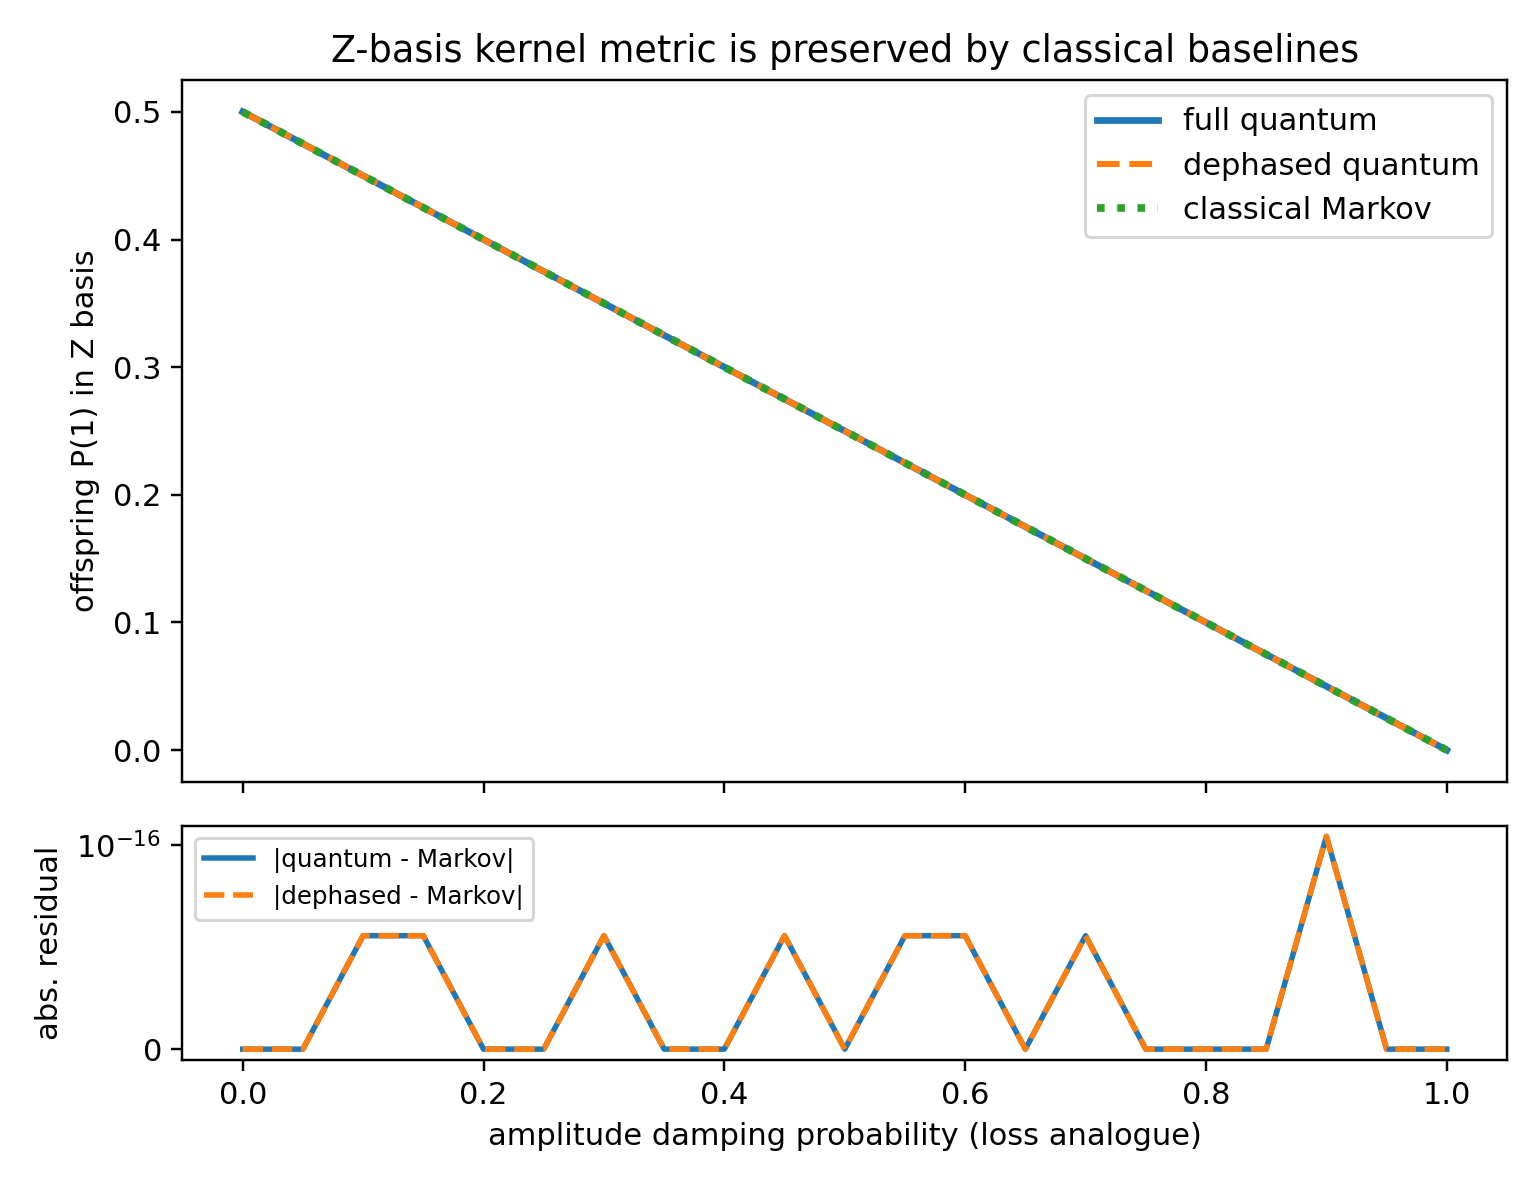
\includegraphics[width=0.78\linewidth]{figures/z_population.png}
\caption{Resource-kernel computational-basis curve for $\theta=\pi/2$ and local-perturbation probability $\mu=0$. The descendant $P(1)$ after damping is identical for the full quantum, dephased quantum, and matched Markov models up to floating-point error.}
\label{fig:zpop}
\end{figure}

\subsection{T2: Noncommuting Diagnostics Identify the Quantum Resource}

Figure~\ref{fig:witnesses} shows the same kernel under noncommuting diagnostics. At zero damping the coherent model reaches negativity $0.5$, concurrence $1.0$, and Horodecki CHSH maximum $2\sqrt{2}\approx2.828$, while dephased and diagonal Markov embeddings have zero negativity and Horodecki CHSH maximum $2.0$. For the $\mu=0$ Bell-damping slice,
\begin{equation}
\mathcal{N}=(1-\gamma)/2,\qquad C=\sqrt{1-\gamma},\qquad S_{\max}=2\sqrt{2(1-\gamma)}.
\end{equation}
The Horodecki CHSH diagnostic reaches the local bound at $\gamma=0.5$. This result is not an experimental Bell test; it is an exact state diagnostic showing which ideal noncommuting correlations the dephased and Markov controls remove.

\begin{figure}[t]
\centering
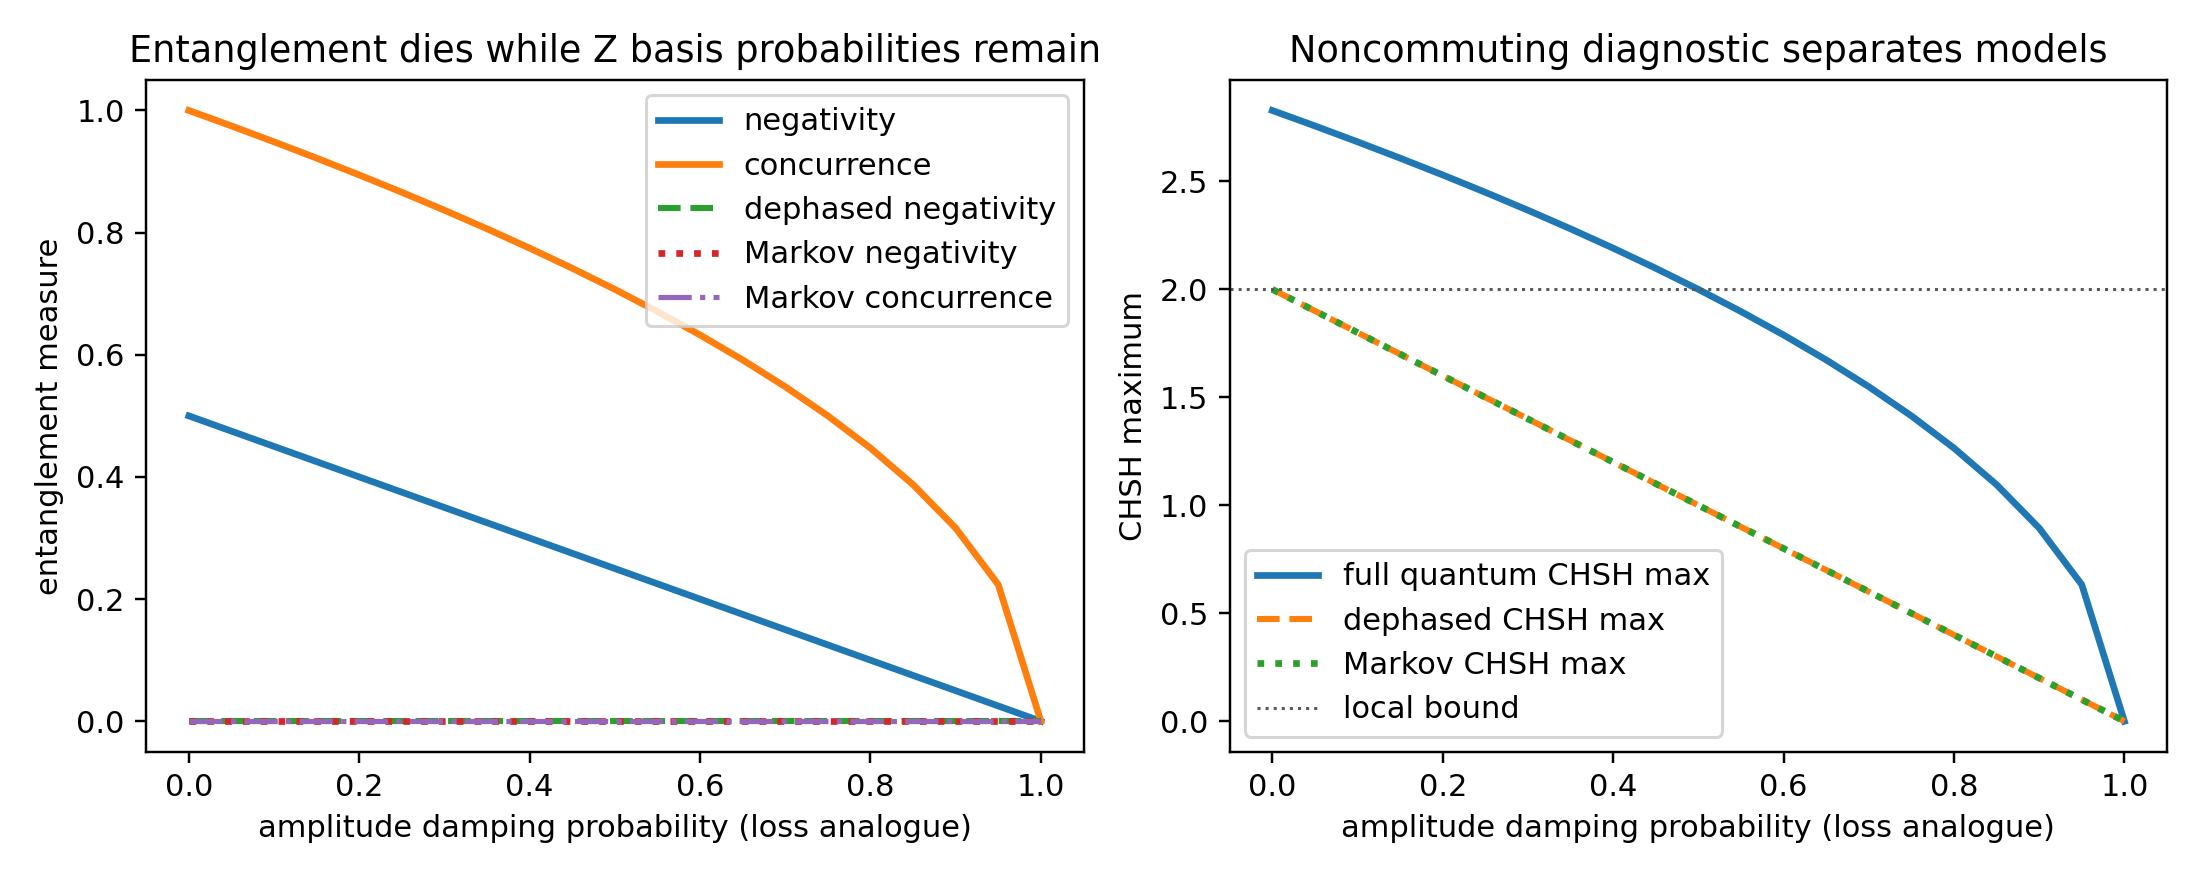
\includegraphics[width=0.86\linewidth]{figures/quantum_diagnostics.png}
\caption{Resource-kernel diagnostics for $\theta=\pi/2$ and $\mu=0$. Entanglement and the ideal Horodecki CHSH value separate the coherent state from dephased and Markov controls even when all computational-basis inheritance metrics remain matched.}
\label{fig:witnesses}
\end{figure}

\subsection{T3: Population Records Establish Selected Reporting Coverage}

The population benchmark records artificial-life quantities that the two-qubit module cannot. In the basis-selection scenario, the quantum, dephased, and classical controls have identical demographic, phenotype, and lineage summaries under matched seeds because selection depends only on basis phenotypes and the event diagonal maps are identical; the resource diagnostics differ by construction. Each of these three controls averages $712.3\pm27.0$ births, $656.3\pm27.0$ deaths, final population $79.98\pm0.20$, maximum lineage depth $16.6\pm1.7$, parent--offspring mutual information $0.00921\pm0.00814$ bits, shuffled-lineage mutual information $0.00102\pm0.00010$ bits, shuffled-null 95th percentile $0.00381\pm0.00055$ bits, parent--child $\theta$ correlation $0.978\pm0.010$, and capacity-blocked opportunity fraction $0.476\pm0.043$ across the 100 basis-selection seeds. The heuristic lineage-MI permutation diagnostic has median empirical $p=0.0149$ across these seeds, with range $0.0050$ to $1.000$; the range is reported because averaging permutation $p$ values is not a useful inference target. The no-inheritance control has similar turnover but collapses continuous genotype-parameter transmission: parent--child $\theta$ correlation falls to $-0.007\pm0.037$ and parent--offspring mutual information falls to $0.00098\pm0.00107$ bits.

These values are deliberately not presented as universal thresholds. They show that QALBench can distinguish reproduction bookkeeping from inherited genotype-parameter transmission and can report a shuffled-lineage diagnostic. The strongest inheritance signal here is the copied $\theta$ parameter; parent--offspring bit mutual information is weak and should be treated as a secondary phenotype-association statistic. Because mutation is applied after the birth phenotype is sampled, mutations affect the genotype used in later descendant events rather than the child phenotype at the same birth event. Figure~\ref{fig:lineage} shows the lineage metrics across all scenarios.

\begin{figure}[t]
\centering
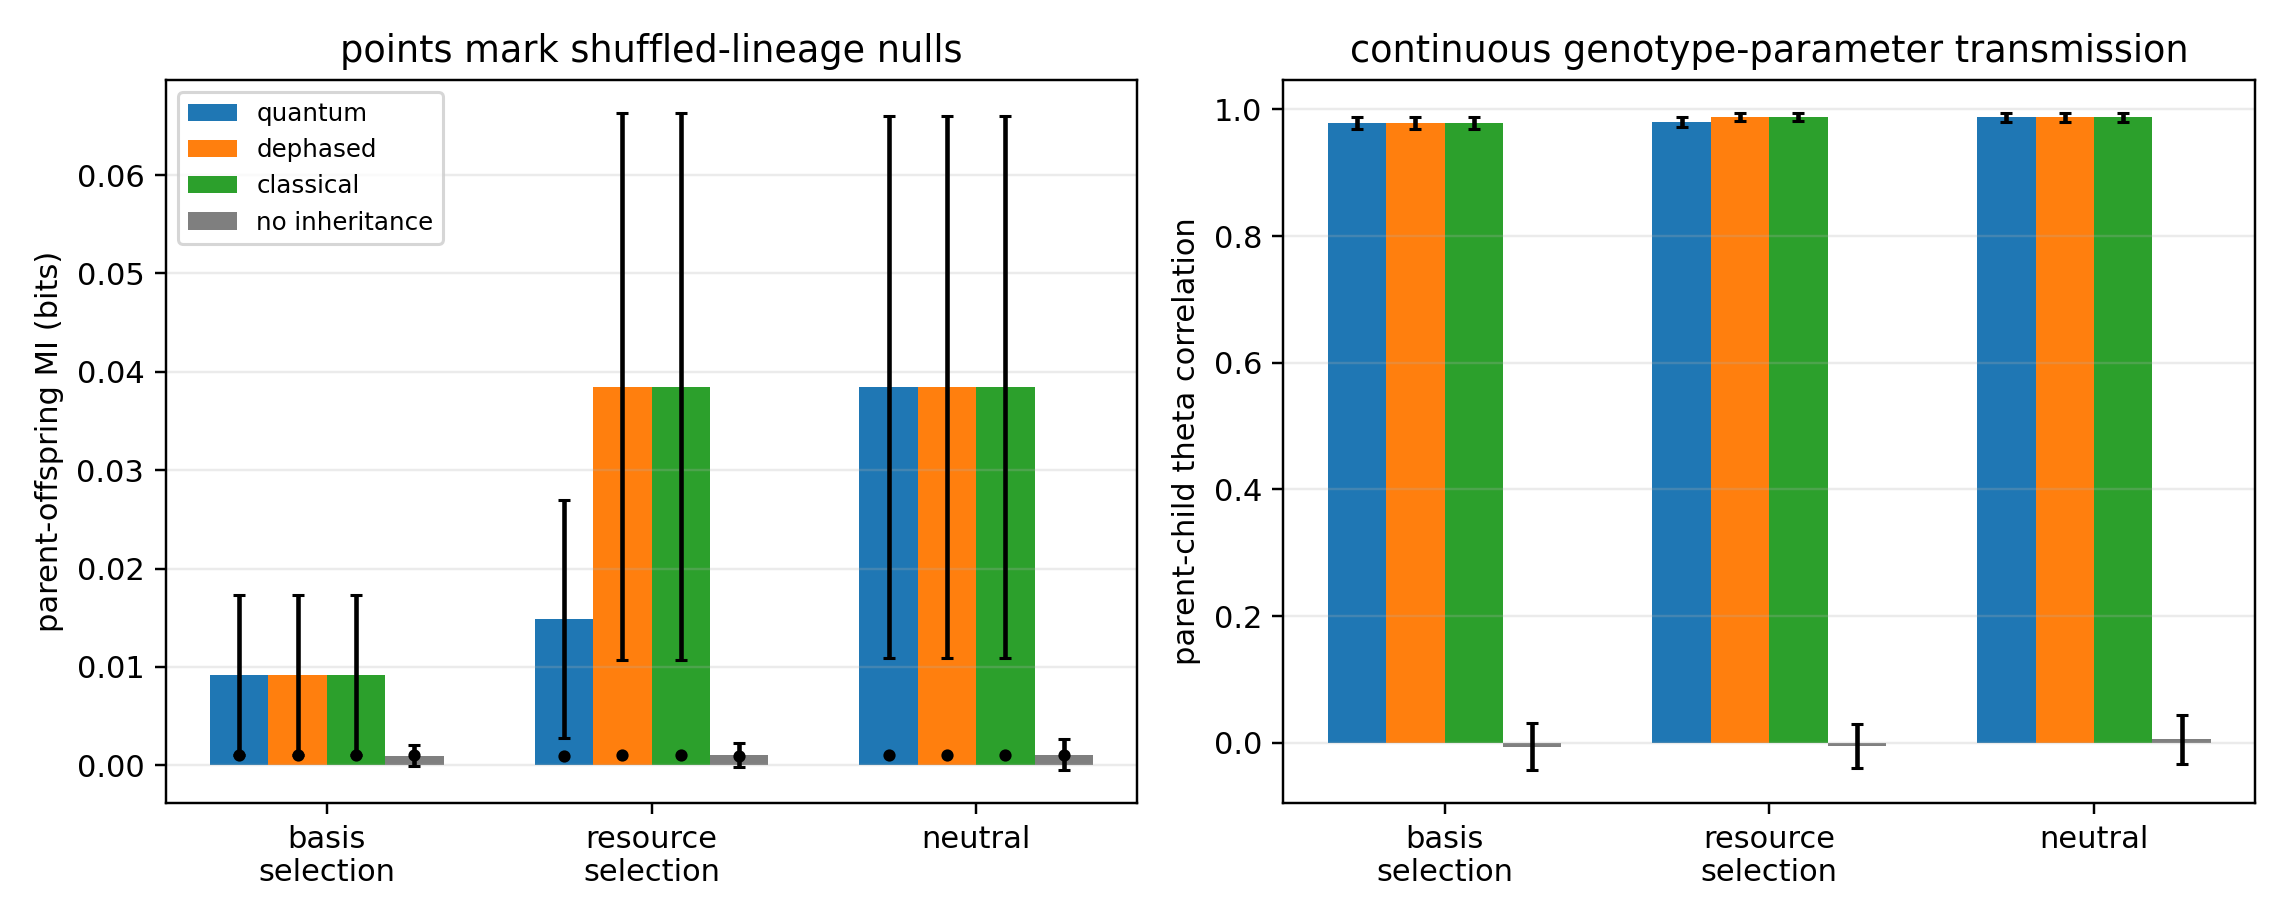
\includegraphics[width=0.94\linewidth]{figures/lineage_nulls.png}
\caption{Population lineage metrics for $n=100$ matched seeds per scenario/model. Bars show means with one-standard-deviation error bars for parent--offspring bit mutual information and parent--child inherited-$\theta$ correlation; black points in the left panel mark the mean of 200 shuffled-lineage mutual-information null permutations per replicate. The no-inheritance control removes continuous genotype-parameter transmission even when births and quantum birth-event resource scores still occur.}
\label{fig:lineage}
\end{figure}

\subsection{T4: Resource-Coupled Positive Control}

Figure~\ref{fig:popoutcomes} summarizes final population and lineage depth. In the basis-selection and neutral scenarios, quantum birth-event resources do not change population outcomes because the selection rule does not use them and the basis probabilities match the Markov map. In the resource positive-control scenario, the benchmark explicitly and synthetically couples reproduction probability to a stored birth-event resource score. This is an engineered software positive-control assay, not evidence that a natural or hardware QAL process would use negativity as a fitness variable. The quantum model then averages birth-event resource score $0.719\pm0.037$ and $744.5\pm25.9$ births per replicate, while dephased and classical controls have zero resource score and $711.8\pm24.6$ births. Using the matched seed labels descriptively, the quantum--classical birth-count difference is $32.7\pm31.3$ births, with median $32.0$ and range $-47$ to $143$ births. This is not treated as a formal paired inference because the stochastic trajectories consume random draws differently after their population histories diverge. The final population remains near carrying capacity for all models; in the resource positive-control quantum run, $0.633\pm0.021$ of parent opportunities are capacity blocked. Birth count, capacity-blocked opportunities, and birth-event resource-score trajectories are therefore more informative than endpoint population alone. Figure~\ref{fig:resource} shows the corresponding time-series birth-event resource scores associated with living individuals.

Table~\ref{tab:population-summary} collects the main population summaries with uncertainty.

\subsection{T3--T4: No-Inheritance Resource Control Is a Negative Result}

The no-inheritance resource control is the key negative result for the population resource assay. It averages resource score $0.635\pm0.008$ and $741.6\pm25.1$ births in the resource positive-control scenario, nearly matching the inherited quantum run in resource-positive reproduction, but its parent--child $\theta$ correlation is only $-0.005\pm0.035$ and its parent--offspring bit mutual information is $0.00105\pm0.00123$ bits. Thus the positive control validates that the inserted resource score can affect reproduction probability; it does not validate inherited resource-mediated artificial life. In the quantum resource positive-control run, parent--child $\theta$ correlation remains high at $0.980\pm0.008$, but parent--offspring bit mutual information is only $0.0149\pm0.0121$ bits and is lower than the dephased/classical value of $0.0385\pm0.0278$ bits. QALBench therefore treats resource-coupled population outcomes, inherited genotype-parameter transmission, and bit-lineage association as separate records. A resource-positive population trace without inherited-state transmission is a failed inheritance claim, even if it is a successful resource-control demonstration.

\begin{table}[t]
\centering
\scriptsize
\setlength{\tabcolsep}{4pt}
\resizebox{\linewidth}{!}{%
\begin{tabular}{lllllll}
\toprule
\textbf{Scenario} & \textbf{Model} & \textbf{Births} & \textbf{Blocked frac.} & \textbf{Resource score} & \textbf{$I(b_p;b_c)$ bits} & \textbf{$\theta$ correlation} \\
\midrule
basis selection & quantum/dephased/classical & $712.3\pm27.0$ & $0.476\pm0.043$ & quantum: $0.492\pm0.124$; controls: $0$ & $0.00921\pm0.00814$ & $0.978\pm0.010$ \\
basis selection & no inheritance & $707.2\pm24.1$ & $0.345\pm0.034$ & $0.635\pm0.007$ & $0.00098\pm0.00107$ & $-0.007\pm0.037$ \\
resource positive control & quantum & $744.5\pm25.9$ & $0.633\pm0.021$ & $0.719\pm0.037$ & $0.0149\pm0.0121$ & $0.980\pm0.008$ \\
resource positive control & dephased/classical & $711.8\pm24.6$ & $0.382\pm0.031$ & $0$ & $0.0385\pm0.0278$ & $0.988\pm0.006$ \\
resource positive control & no inheritance & $741.6\pm25.1$ & $0.618\pm0.019$ & $0.635\pm0.008$ & $0.00105\pm0.00123$ & $-0.005\pm0.035$ \\
neutral & quantum/dephased/classical & $711.0\pm25.9$ & $0.382\pm0.032$ & quantum: $0.625\pm0.082$; controls: $0$ & $0.0385\pm0.0275$ & $0.988\pm0.007$ \\
neutral & no inheritance & $708.7\pm23.3$ & $0.384\pm0.029$ & $0.637\pm0.006$ & $0.00107\pm0.00158$ & $0.005\pm0.038$ \\
\bottomrule
\end{tabular}
}
\caption{Default population summary. Values are mean $\pm$ standard deviation over $n=100$ matched seeds. Grouped quantum/dephased/classical rows have identical demographic, phenotype, and lineage summaries under matched seeds; resource-score entries are split because only coherent quantum birth events have nonzero negativity. Blocked fraction is the fraction of post-death parent opportunities blocked by carrying capacity. The full artifact also contains deaths, final population, lineage depth, diversity, mutation, opportunity-level mean birth probability, selection-gradient diagnostics, and interaction-covariance fields.}
\label{tab:population-summary}
\end{table}

\begin{table}[t]
\centering
\scriptsize
\setlength{\tabcolsep}{4pt}
\begin{tabular}{lllll}
\toprule
\textbf{Seeds} & \textbf{Basis $\theta$ corr.} & \textbf{No-inheritance $\theta$ corr.} & \textbf{Resource birth diff.} & \textbf{Resource score} \\
\midrule
10 & $0.978\pm0.009$ & $0.003\pm0.029$ & $32.7\pm33.0$ & $0.717\pm0.041$ \\
30 & $0.977\pm0.012$ & $-0.003\pm0.035$ & $27.0\pm27.6$ & $0.714\pm0.043$ \\
50 & $0.977\pm0.010$ & $-0.003\pm0.033$ & $29.7\pm28.3$ & $0.718\pm0.037$ \\
100 & $0.978\pm0.010$ & $-0.007\pm0.037$ & $32.7\pm31.3$ & $0.719\pm0.037$ \\
\bottomrule
\end{tabular}
\caption{Cumulative seed-count sensitivity for selected population diagnostics, using seeds 11 through $10+n$. Values are mean $\pm$ standard deviation. The resource birth difference is the descriptive matched-seed quantum-minus-classical birth-count difference in the resource positive-control scenario; resource score is the quantum mean event-resource score in that scenario. Across all four cumulative subsets, basis-selection quantum and classical birth counts are identical under matched seeds.}
\label{tab:seed-sensitivity}
\end{table}

\begin{figure}[t]
\centering
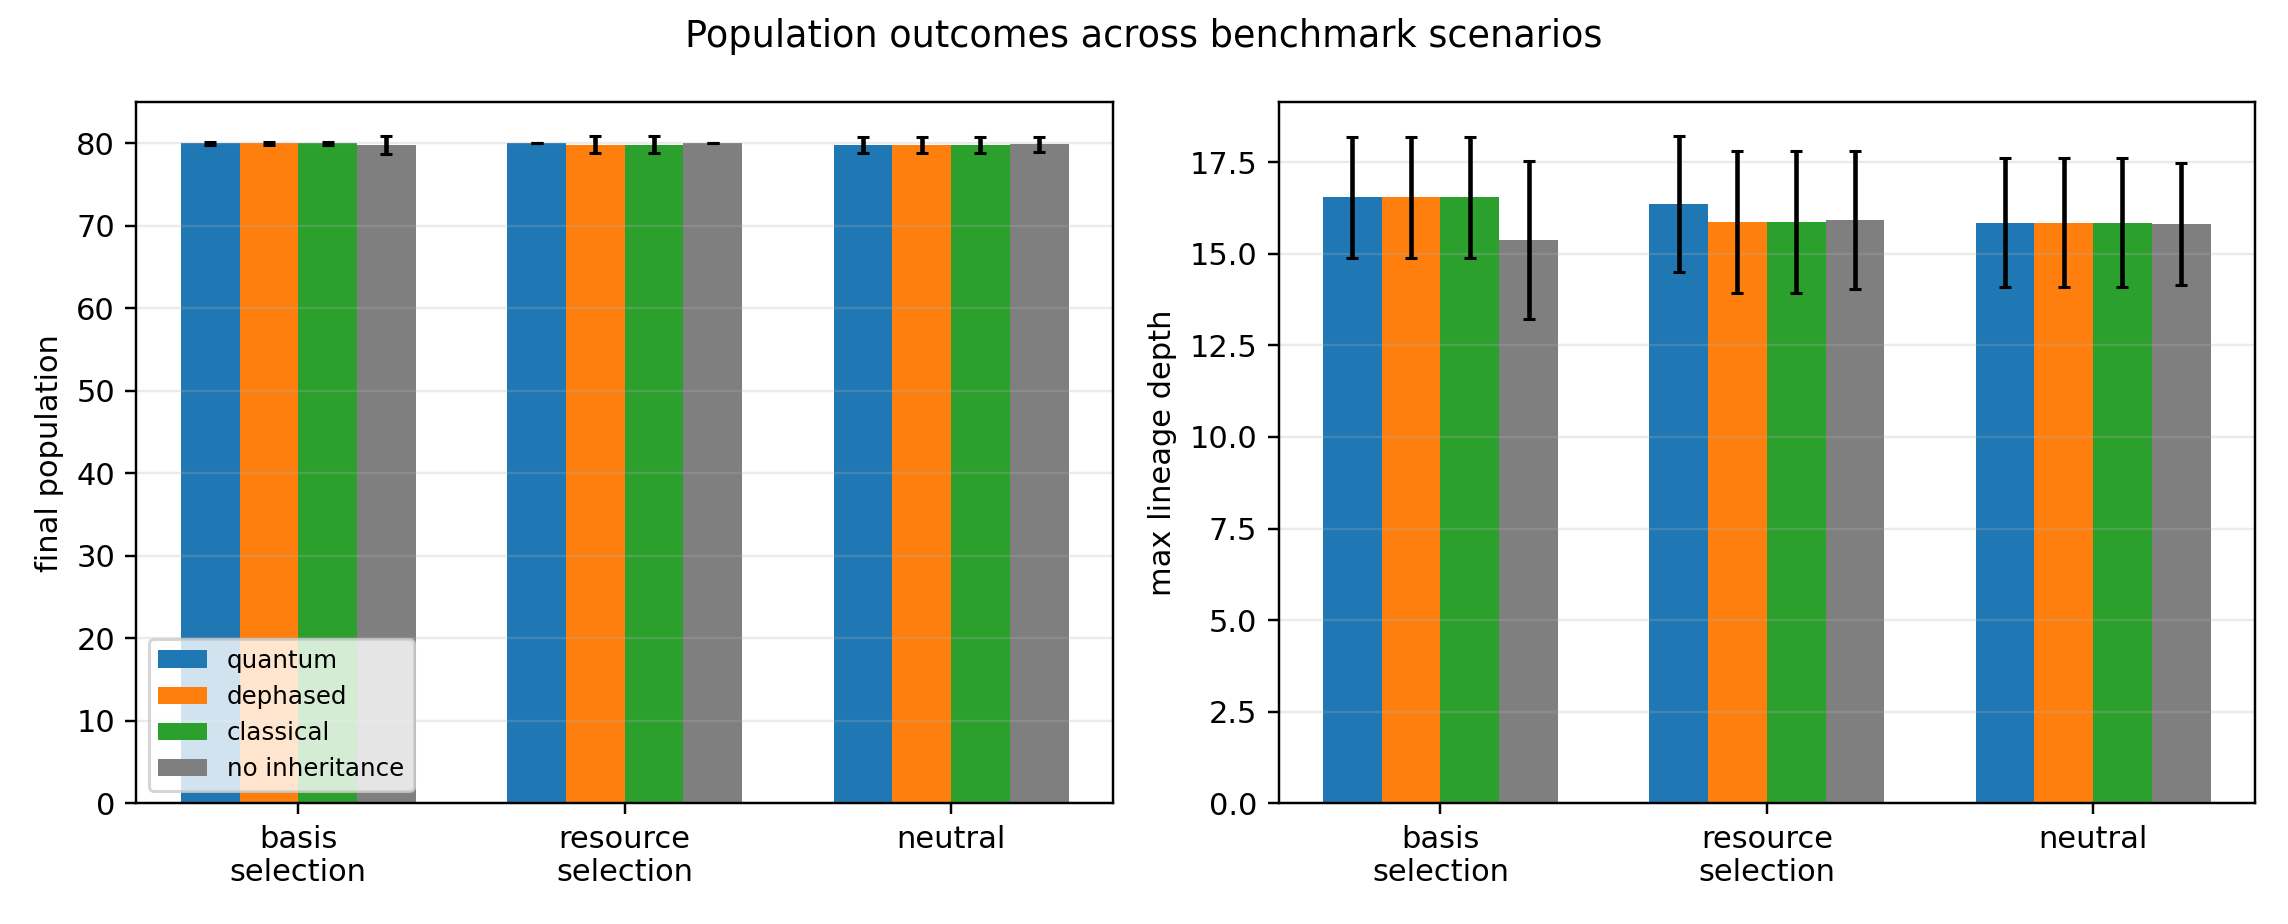
\includegraphics[width=0.94\linewidth]{figures/population_outcomes.png}
\caption{Population outcomes across benchmark scenarios for $n=100$ matched seeds per scenario/model. Bars show means with one-standard-deviation error bars; the full CSV preserves seed-level rows for uncertainty checks. Basis-selection demographic, phenotype, and lineage outcomes are identical for quantum, dephased, and classical controls under matched seeds because only computational-basis phenotypes affect reproduction. The resource positive-control scenario is an engineered positive control in which birth dynamics change when a nonzero birth-event resource score is inserted into the reproduction rule.}
\label{fig:popoutcomes}
\end{figure}

\begin{figure}[t]
\centering
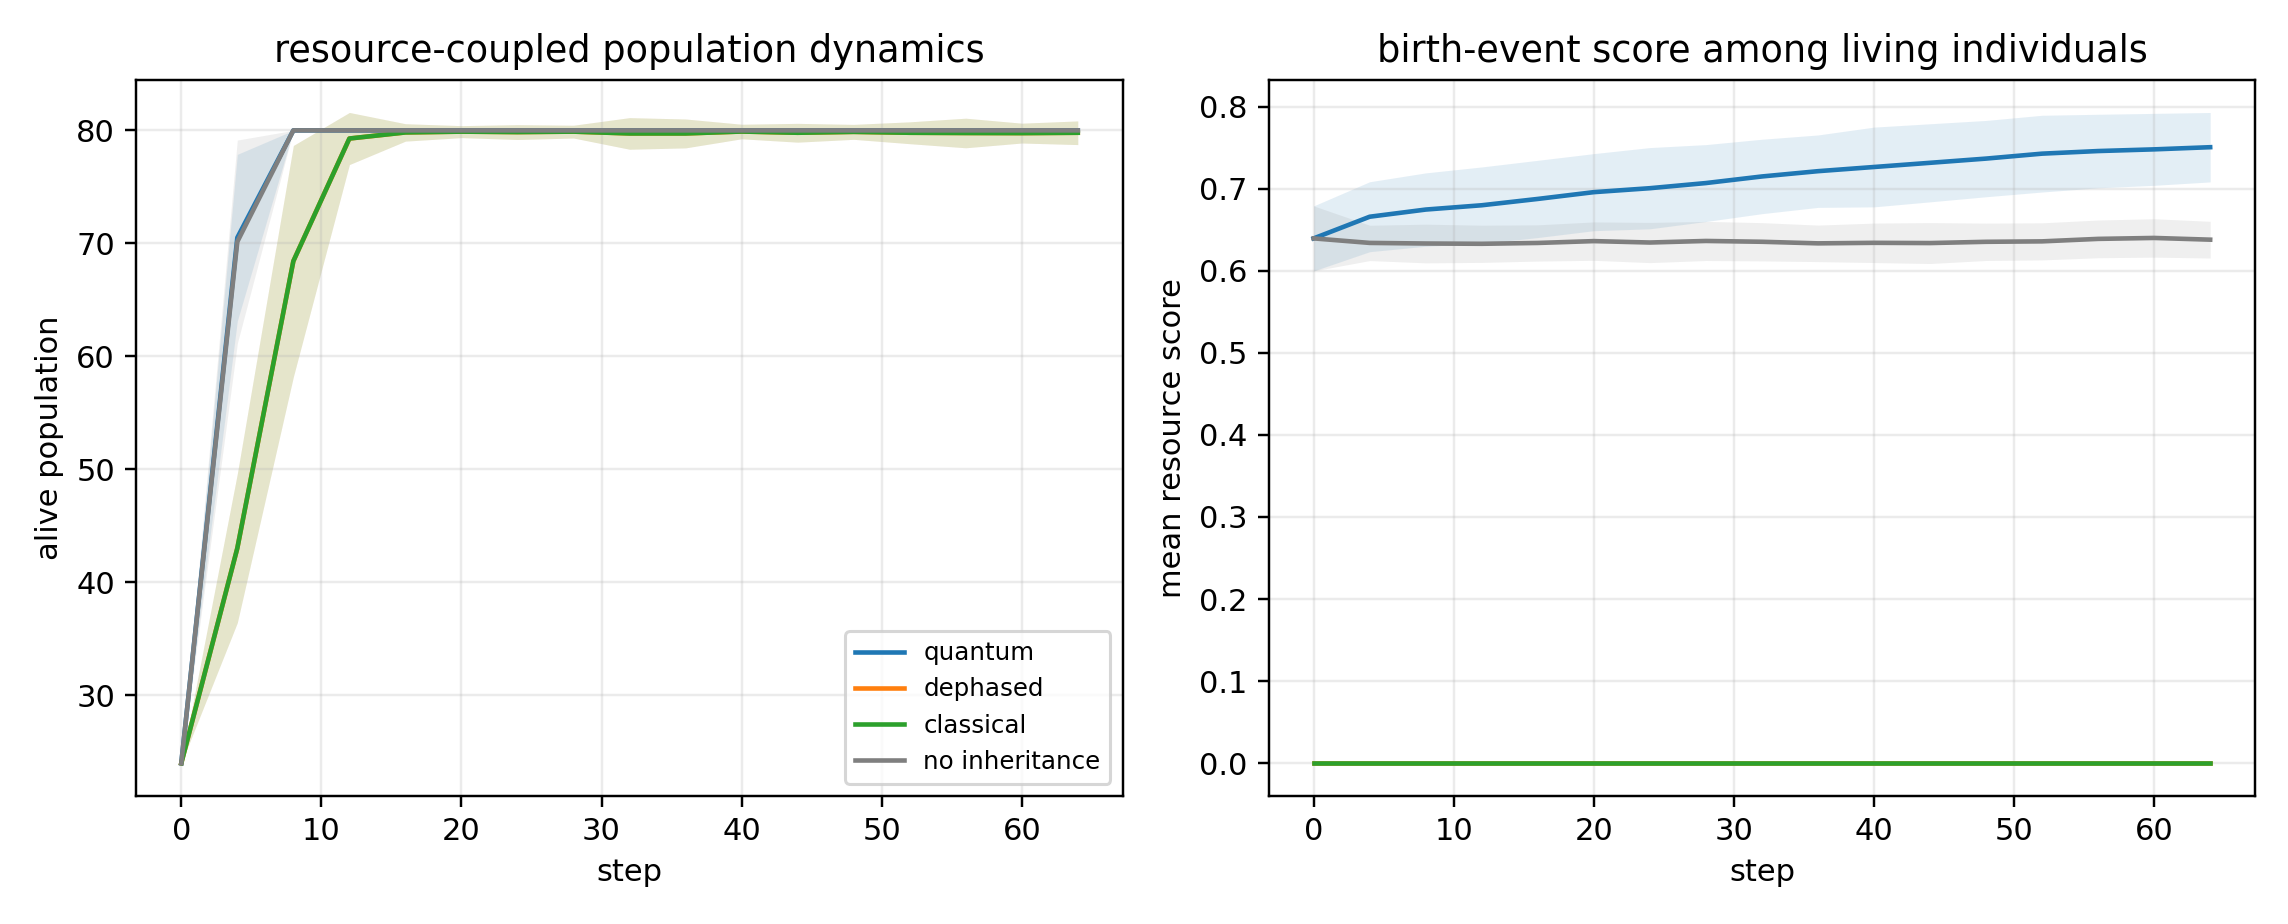
\includegraphics[width=0.94\linewidth]{figures/resource_relevance.png}
\caption{Resource-coupled positive-control scenario over time for $n=100$ matched seeds. Lines show means and shaded bands show one standard deviation. The plotted resource quantity is the mean birth-event resource score associated with currently living individuals; it is not persistent population-level entanglement or coherence. Dephased and classical controls have zero negativity-derived resource score. Population size saturates near carrying capacity, so the benchmark also reports births, capacity-blocked opportunities, lineages, and transmission metrics.}
\label{fig:resource}
\end{figure}

\FloatBarrier

\section{Audit Examples on Prior QAL Work}

Table~\ref{tab:coverage} shows how the audit vocabulary can be applied to three illustrative QAL-associated papers. The table is not an adjudication of paper quality, a priority claim, or a complete field survey; it is limited to papers that use QAL-style inheritance, self-replication, or organism language rather than the broader set of quantum cellular automata, quantum simulation benchmarks, artificial chemistry, or quantum-biology models. It separates what the papers report from additional controls that would be needed for stronger population, resource-certification, or computational-nonclassicality claims. Open-ended-evolution metric work motivates the reporting rows for novelty, diversity, and adaptation \citep{bullock2006exploring,banzhaf2016defining,packard2019overview,dolson2019modes}, while quantum cellular-automaton and quantum Game-of-Life studies motivate future many-body modules \citep{bleh2012quantum,ney2022entanglement,escanez2026qgol}. QALBench does not subsume those areas; it targets claim-specific audits for QAL papers that use inheritance, lineage, selection, and quantum-resource language together.

\begin{table}[!htbp]
\centering
\scriptsize
\setlength{\tabcolsep}{3.5pt}
\begin{tabular}{P{0.18\linewidth}P{0.38\linewidth}P{0.34\linewidth}}
\toprule
\textbf{Paper} & \textbf{Reported elements matching audit rows} & \textbf{Additional controls for stronger claims} \\
\midrule
\citet{alvarez2016artificial} & Defines genotype/phenotype quantum living units, self-replication by partial $\sz$ cloning, mutation, spatial motion, genotype-conditioned interaction, and Lindblad phenotype aging/death. Provides small simulated histories. & Stronger inherited-resource or computational claims would require claim-matched Markov/dephased controls for basis observables, scalable lineage bookkeeping, finite-shot resource certificates, and computational-simulation baselines. \\
\addlinespace
\citet{alvarez2018ibm} & Implements small IBM hardware subprotocols for $\sz$ replication, mutation cases, dissipative phenotype dynamics, and interaction circuits. Explicitly discusses classical reproducibility of $\sz$ indicators and quantum genealogical correlations. & Stronger population-level artificial-life claims would require birth/death/lineage scaling, and stronger resource claims would require SPAM-aware finite-shot entanglement witnesses or Bell-test certification. \\
\addlinespace
\citet{valente2021self} & Gives a thermodynamic single-photon self-replication mechanism with replication probabilities, work absorption, and rare mutation transitions. & Stronger QAL claims would require population-level artificial-life records, resource-destroying controls tied to the claimed outcome, and operational certification if entanglement, nonlocality, contextuality, or computational nonclassicality is asserted. \\
\bottomrule
\end{tabular}
\caption{Illustrative audit reading of representative QAL papers. The right column lists controls that would be needed only for stronger claims than the reported evidence directly supports.}
\label{tab:coverage}
\end{table}

\FloatBarrier

\section{Limitations and Claim Boundary}

QALBench answers two questions that the original resource-kernel audit did not fully answer. First, it asks whether artificial-life claims survive population records and nulls. The population module computes parent IDs, generations, inherited genotype parameters, expressed bits, births, deaths, inherited-model mutations, sampled interaction exposures, reproduction opportunities, capacity-blocked opportunities, imposed selection-rule outcomes, lineage mutual information, shuffled-lineage diagnostics, and no-inheritance controls. These records establish coverage of selected reporting fields, not open-ended artificial life or adaptation in the stronger sense. Second, it asks whether a claimed quantum-resource dependence can be made removable by an appropriate control. The basis-selection scenario shows that quantum, dephased, and classical variants can have identical non-resource population summaries when the outcome depends only on the cloned computational-basis observable. The resource positive-control scenario shows how to define a software outcome coupled to a stored event-level resource score, remove the score with controls, quantify descriptive uncertainty under matched seed labels, and still require lineage transmission to support artificial-life language.

The benchmark is intentionally modular. A hardware T5 submission can now use the suite's count, certificate, and calibration schema, but it must supply real counts, readout assumptions, controls, and witness or Bell-test protocol details before a hardware-specific claim is scored. A population submission can replace the synthetic selection rule with platform-specific survival, replication, or energy-flow mechanisms. The benchmark demand remains the same: state the artificial-life claim, state the quantum-resource claim, run the corresponding nulls, and report which claims survive.

In the tier language of Table~\ref{tab:tiers}, the present resource-kernel artifacts instantiate T1 and T2, the population records instantiate T3, and the resource-selection scenario instantiates T4 only as a software positive control. The suite infrastructure additionally implements T5 and T6 submission contracts, reference packages, validators, and scorers. This framing is meant to make partial submissions comparable without flattening them into a single score. A hardware experiment with finite-shot witnesses would add positive T5 evidence only when the submitted counts and calibration records pass the relevant checks. A scalable simulation challenge would add positive T6 evidence only when the task output, error model, classical simulator families, size coverage, and compute disclosures pass the nonclassicality validator.

The population module is not a many-body quantum simulation of all individuals. It is a population-level reporting benchmark with event-level quantum-resource diagnostics attached to otherwise classical individuals. No quantum state, entanglement, or coherence is inherited through the population. This is a deliberate engineering choice: exact density matrices over a growing population scale exponentially and would obscure the claim-specific controls. The resource positive-control scenario is also synthetic; it demonstrates a software positive-control assay for an explicitly resource-coupled outcome, not that a particular physical organism would use negativity as a fitness variable. The default population artifact uses 100 matched seeds per scenario/model, with a cumulative seed-count sensitivity table for selected diagnostics. This is enough to stabilize the benchmark's qualitative checks, but the matched seed labels do not by themselves create a formal paired experiment once trajectories diverge. The shuffled-lineage diagnostic reports 200 permutations per replicate, but stronger inference would still benefit from lineage-aware nulls, additional stochastic replicates for specific effect-size claims, and model sensitivity analysis. The default artifact records interaction exposures but lacks a randomized-neighbor control for controlled interaction-effect claims. The canonical numerical artifacts do not model a spatial grid, open-ended novelty, resource metabolism, finite-shot hardware noise, process tomography, or quantum advantage. The suite layer now includes finite-shot/readout schemas and small-system simulator-baseline workflows, but not external hardware evidence, device-independent certification, asymptotic hardness evidence, or positive quantum-advantage results.

\section{Conclusion}

QALBench turns QAL reporting into a tiered set of claim-specific audit tasks. In the cloned-observable resource kernel, computational-basis inheritance metrics are exactly reproduced by dephased and Markov controls, while noncommuting diagnostics reveal the quantum resource. In the population module, lineage records, no-inheritance controls, shuffled-lineage diagnostics, turnover, mutation, interaction-exposure records, and selection-rule metrics distinguish artificial-life reporting coverage from event-level resource presence. The suite layer extends that conservative audit stance to T5 and T6 by requiring finite-shot certificates, calibration records, simulator baselines, scaling specifications, compute disclosures, and explicit nonclassicality evidence before stronger axes can score. The benchmark result is conservative but useful: basis-only outcomes in cloned-observable protocols of this type should be checked against matched classical controls; quantum-resource claims should be tied to operational diagnostics or certificates; population-level claims should report lineage and null records; and stronger hardware or computational claims should be audited as higher-tier submissions rather than inferred from lower-tier evidence.

\section*{Data and Code Availability}

The QALBench implementation used for this draft is publicly available under the MIT license at \url{https://github.com/Gabriel-Kahen/qal-bench}. The archival software release \texttt{v0.3.0}, deposited on Zenodo at \url{https://zenodo.org/records/20222166} with version DOI \href{https://doi.org/10.5281/zenodo.20222166}{10.5281/zenodo.20222166}, contains the T1--T6 suite layer described in this draft and supports the canonical T1--T4 numerical artifacts and figures reported here. The Zenodo concept DOI for all versions is \href{https://doi.org/10.5281/zenodo.20215830}{10.5281/zenodo.20215830}.

The canonical resource-kernel artifacts are the sweep CSV, sweep metadata JSON, and associated figures under \path{results/}; paper copies of figures are synced under \path{paper/figures/}. These artifacts support the reported T1--T2 numerical results. The phase-diagram figure is included as an artifact-level diagnostic for the full resource-kernel sweep but is not used as a main-text result. The current T3--T4 population artifacts are:
\begin{itemize}
\item \path{results/qalbench_population.csv}
\item \path{results/qalbench_population_timeseries.csv}
\item \path{results/qalbench_population_individuals.csv.xz}
\item \path{results/qalbench_population_attempts.csv.xz}
\item \path{results/qalbench_population_birth_events.csv.xz}
\item \path{results/qalbench_population_metadata.json}
\end{itemize}
The verifier scripts recompute the numerical rows from the implementation, check schemas, check parameter coverage, validate source-file manifests, and check CSV and figure hashes. The suite-layer documentation and checks for general submissions are in \path{docs/submission_schema.md} and \path{docs/suite_completion_audit.md}; the command-line entry point is \texttt{qalbench-suite}.

The audit path for existing checked-in artifacts is \texttt{scripts/verify\_release\_artifacts.sh}. The regeneration path is \texttt{scripts/reproduce\_all.sh}, which runs the unit tests, regenerates the resource-kernel and population artifacts, verifies them, and rebuilds the PDF when Tectonic is installed. The tagged release was verified with version-consistent metadata before archival deposit.

\bibliographystyle{unsrtnat}
\bibliography{references}

\end{document}
